\chapter{Część teoretyczna}\label{chap:teoria}
Ten rozdział powinien zawierać teorię z~której autor będzie korzystał w~dalszej
części pracy.  Podstawowym celem istnieniem tego rozdziału jest umożliwienie
czytelnikowi zrozumienie teorii rozwijanej w pracy oraz osiągniętych wyników
praktycznych.  Jeżeli jakieś informacje nie są niezbędne do zrozumienia
osiągnięć autora nie należy o nich pisać.

\section{Architektura Glasgow Haskell Compiler}

\todo[inline]{Treść. Kompilator. Rysunek z AOSA. Frontend i backend.}

\begin{figure}[ht]
    \centering
    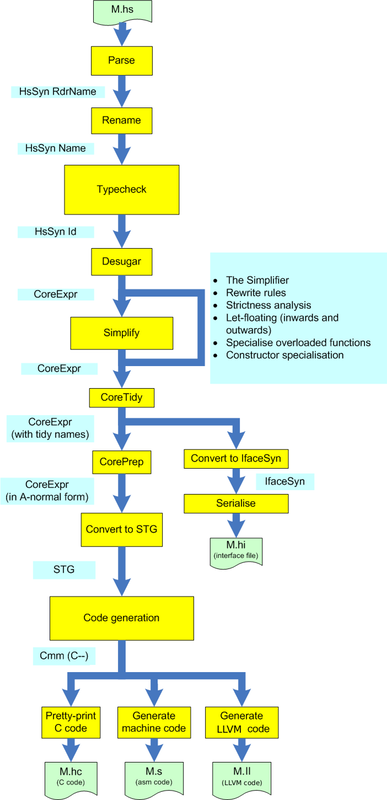
\includegraphics[width=0.8\textwidth]{images/AOSA_compiler}
    \caption[Schemat Glasgow Haskell Compiler]{Schemat Glasgow Haskell Compiler\cite{AOSA}}
    \label{fig:AOSA_compiler}
\end{figure}

\subsection{Parser}
\todo[inline]{Treść, raczej pod kątem zgłoszenia z \code{NamedWildCards}}

\subsection{Renamer}
\todo[inline]{Treść, pod \code{-fwarn-unused-matches} i \code{NamedWildCards}.}

\subsection{Type checker}
\todo[inline]{Treść, pod pierwsze zgłoszenie?}

\section{Rozszerzenia GHC}

\todo[inline]{Standard Haskell. Liczba rozszerzeń. Było to już we wstępie.}

\subsectionex{Rodziny typów}{Rozszerzenie \code{TypeFamilies}}
\todo[inline]{Treść zaczerpnięta z UsersGuide\cite{GuideTypeFamilies}. Pamiętać o \code{DataFamilies}}

\subsectionex{Częściowe sygnatury typów}{Rozszerzenie \code{PartialTypeSignatures}}
\todo[inline]{Treść zaczerpnięta z UsersGuide\cite{GuidePartialTypeSignatures}. Pamiętać o \code{NamedWildCards}}
